%% abtex2-modelo-relatorio-tecnico.tex, v<VERSION> laurocesar
%% Copyright 2012-2015 by abnTeX2 group at http://www.abntex.net.br/ 
%%
%% This work may be distributed and/or modified under the
%% conditions of the LaTeX Project Public License, either version 1.3
%% of this license or (at your option) any later version.
%% The latest version of this license is in
%%   http://www.latex-project.org/lppl.txt
%% and version 1.3 or later is part of all distributions of LaTeX
%% version 2005/12/01 or later.
%%
%% This work has the LPPL maintenance status `maintained'.
%% 
%% The Current Maintainer of this work is the abnTeX2 team, led
%% by Lauro César Araujo. Further information are available on 
%% http://www.abntex.net.br/
%%
%% This work consists of the files abntex2-modelo-relatorio-tecnico.tex,
%% abntex2-modelo-include-comandos and abntex2-modelo-references.bib
%%

% ------------------------------------------------------------------------
% ------------------------------------------------------------------------
% abnTeX2: Modelo de Relatório Técnico/Acadêmico em conformidade com 
% ABNT NBR 10719:2011 Informação e documentação - Relatório técnico e/ou
% científico - Apresentação
% Adaptado por Daniel Saad Nogueira Nunes para uso no IFB Taguatinga.
% ------------------------------------------------------------------------ 
% ------------------------------------------------------------------------


% Como opção escolha 'bacharelado' ou 'licenciatura'
\documentclass[bacharelado]{pre-projeto-computacao}
% ---
% Informações de dados para CAPA e FOLHA DE ROSTO
% ---
\titulo{Estudo experimental: Avaliação comparativa de alternativas ao MinIO para armazenamento de objetos em arquiteturas de data lake híbridas}
\autor{Erick Sousa Saraiva}

% para feminino use \orientadora{Nome da orientadora}
\orientador{Fabiano Cavalcanti Fernandes}

% para masculino use \coorientador{Nome do coorientador}
\coorientadora{}

% Linha de pesquisa conforme tabela de áreas do CNPq
\areadepesquisa{Sistemas Distribuídos}
\local{Brasília, DF}
\data{19 de junho de 2026}

\begin{document}

\selectlanguage{brazil}
\frenchspacing 
\imprimircapa
\imprimirfolhaderosto



\section*{Contextualização}

A crescente demanda por processamento e análise de grandes volumes de dados
impulsionou a adoção de arquiteturas de \textit{Data Lake}, que permitem o
armazenamento centralizado de dados brutos em diferentes formatos:
estruturados, semiestruturados e não estruturados, sem necessidade de
transformação prévia \cite{tast2026comparative}. Nesse sentido, o armazenamento é
desacoplado do processamento, favorecendo flexibilidade e escalabilidade, e sendo
amplamente utilizado em pipelines de aprendizado de máquina e análise de dados
em larga escala, o data lake atua como repositório central para dados de diferentes
fontes, videos, imagens, documento e etc...

Em cenários de nuvem híbrida, organizações que buscam mitigar riscos de soberania
de dados e de dependência de fornecedor (\textit{vendor lock-in}) optam por manter
parte da infraestrutura de armazenamento \textit{on-premises}, replicando
funcionalidades oferecidas por provedores como Amazon Web Services (AWS), Microsoft
Azure e Google Cloud Platform (GCP), basicamente sendo uma solução de armazenamento
local e distribuído sem precisar de infraestrutura em nuvem. A camada de armazenamento
de objetos é componente central nessas arquiteturas, e o protocolo S3 da AWS
consolidou-se como padrão de fato para interoperabilidade entre sistemas
\cite{tast2026comparative}.

Nesse contexto, o MinIO tornou-se uma solução amplamente utilizada para
armazenamento de objetos compatível com a API S3 em arquiteturas de \textit{Data Lake}
híbridas \cite{abdel2026pipeline}. Ao longo dos anos, a empresa responsável pelo
projeto promoveu mudanças progressivas em seu modelo de distribuição e licenciamento:
em 2021, a licença foi alterada de Apache 2.0 para GNU AGPLv3; em maio de 2025, a
interface de administração web foi removida da edição comunitária; em outubro de
2025, as distribuições binárias pré-compiladas foram descontinuadas, passando a
edição comunitária a ser distribuída apenas como código-fonte; e em fevereiro de
2026, o repositório público foi oficialmente marcado como não mantido
(\textit{THIS REPOSITORY IS NO LONGER MAINTAINED}), com correções de segurança
passando a ser avaliadas caso a caso, sem garantias \cite{minio2026repo,
devpro2025, faun2026}. O suporte ativo, os binários e as funcionalidades completas
de administração foram concentrados no produto comercial MinIO AIStor, disponível
por assinatura.

Esse cenário expõe organizações que basearam sua camada de armazenamento de objetos
no MinIO a riscos concretos de segurança, de conformidade e de sustentabilidade
tecnológica, tornando relevante a avaliação de alternativas viáveis com licenciamento
aberto e compatibilidade com a API S3, e também a governança de dados, para mitigar
riscos de dependência tecnológica e de \textit{vendor lock-in}.


\section*{Proposta}

Este trabalho propõe um estudo experimental para avaliar comparativamente ao menos
três soluções de armazenamento de objetos compatíveis com a API S3, utilizando o
MinIO como \textit{baseline} de referência, sendo o RustFS uma das alternativas
obrigatoriamente incluídas. As demais soluções serão selecionadas durante o
levantamento bibliográfico, priorizando projetos com licenciamento aberto e
adoção ativa pela comunidade.

O objetivo geral é avaliar comparativamente alternativas ao MinIO para
armazenamento de objetos em arquiteturas de \textit{Data Lake} híbridas,
considerando aspectos de desempenho, compatibilidade com a API S3,
interoperabilidade com provedores de nuvem, custos, licenciamento,
sustentabilidade e riscos tecnológicos.

São objetivos específicos deste trabalho:

\begin{itemize}
    \item Identificar soluções de armazenamento de objetos compatíveis com a
          API S3 que possam constituir alternativas ao MinIO em arquiteturas
          híbridas;
    \item Caracterizar os requisitos técnicos relevantes para armazenamento de
          objetos em arquiteturas de \textit{Data Lake} híbridas;
    \item Implementar um ambiente experimental padronizado para implantação e
          avaliação das soluções selecionadas;
    \item Investigar a compatibilidade das soluções com a API S3 e sua
          interoperabilidade com serviços de nuvem (AWS, Azure e GCP);
    \item Avaliar o desempenho e o consumo de recursos das soluções em cenários
          controlados com conjuntos de dados de diferentes características;
    \item Analisar comparativamente as soluções segundo custos, modelo de
          licenciamento, maturidade do projeto e riscos tecnológicos.
\end{itemize}


\section*{Justificativa}

As mudanças progressivas no modelo de distribuição e licenciamento do MinIO
representam um risco concreto para organizações públicas e privadas que adotaram
a solução como componente central de sua infraestrutura de dados. A descontinuação
das distribuições binárias e o congelamento do desenvolvimento comunitário em 2025,
seguidos pelo arquivamento do repositório público em fevereiro de 2026
\cite{faun2026, minio2026repo}, comprometem a previsibilidade operacional de
ambientes que dependem da solução, especialmente em contextos de nuvem híbrida
onde soberania de dados e controle sobre a infraestrutura são requisitos críticos, em
organizações públicas, por exemplo.

A ausência de estudos comparativos publicados que avaliem alternativas ao MinIO
nesse cenário específico --- considerando soluções emergentes como o RustFS e
aspectos como compatibilidade com provedores de nuvem, sustentabilidade do
licenciamento e riscos de dependência tecnológica --- justifica a relevância
acadêmica desta pesquisa \cite{tast2026comparative}. Os resultados poderão
orientar equipes de engenharia de dados na seleção de tecnologias mais sustentáveis,
contribuindo para a redução de riscos de segurança e de \textit{vendor lock-in}.


\section*{Proposta Metodológica Preliminar}

A pesquisa será conduzida em duas grandes etapas: um mapeamento sistemático da
literatura, que fornecerá o fundamento teórico e subsidiará a definição dos critérios
de avaliação no laboratório prático, o qual será o objeto principal de estudo da referente pesquisa e um estudo experimental comparativo, com o MinIO como
\textit{baseline} de referência. A pesquisa está estruturada em cinco fases:

\textbf{Fase 1 --- Mapeamento sistemático da literatura.}
Realização de um mapeamento sistemático com o objetivo de identificar o que a
literatura científica aponta como dimensões, métricas e critérios relevantes para
avaliação de soluções de armazenamento de objetos em contextos de \textit{data lake}
híbrido. O mapeamento seguirá as diretrizes de \cite{kitchenham2010}, estruturado
nas seguintes etapas:
\begin{figure}[htb]
    \centering
    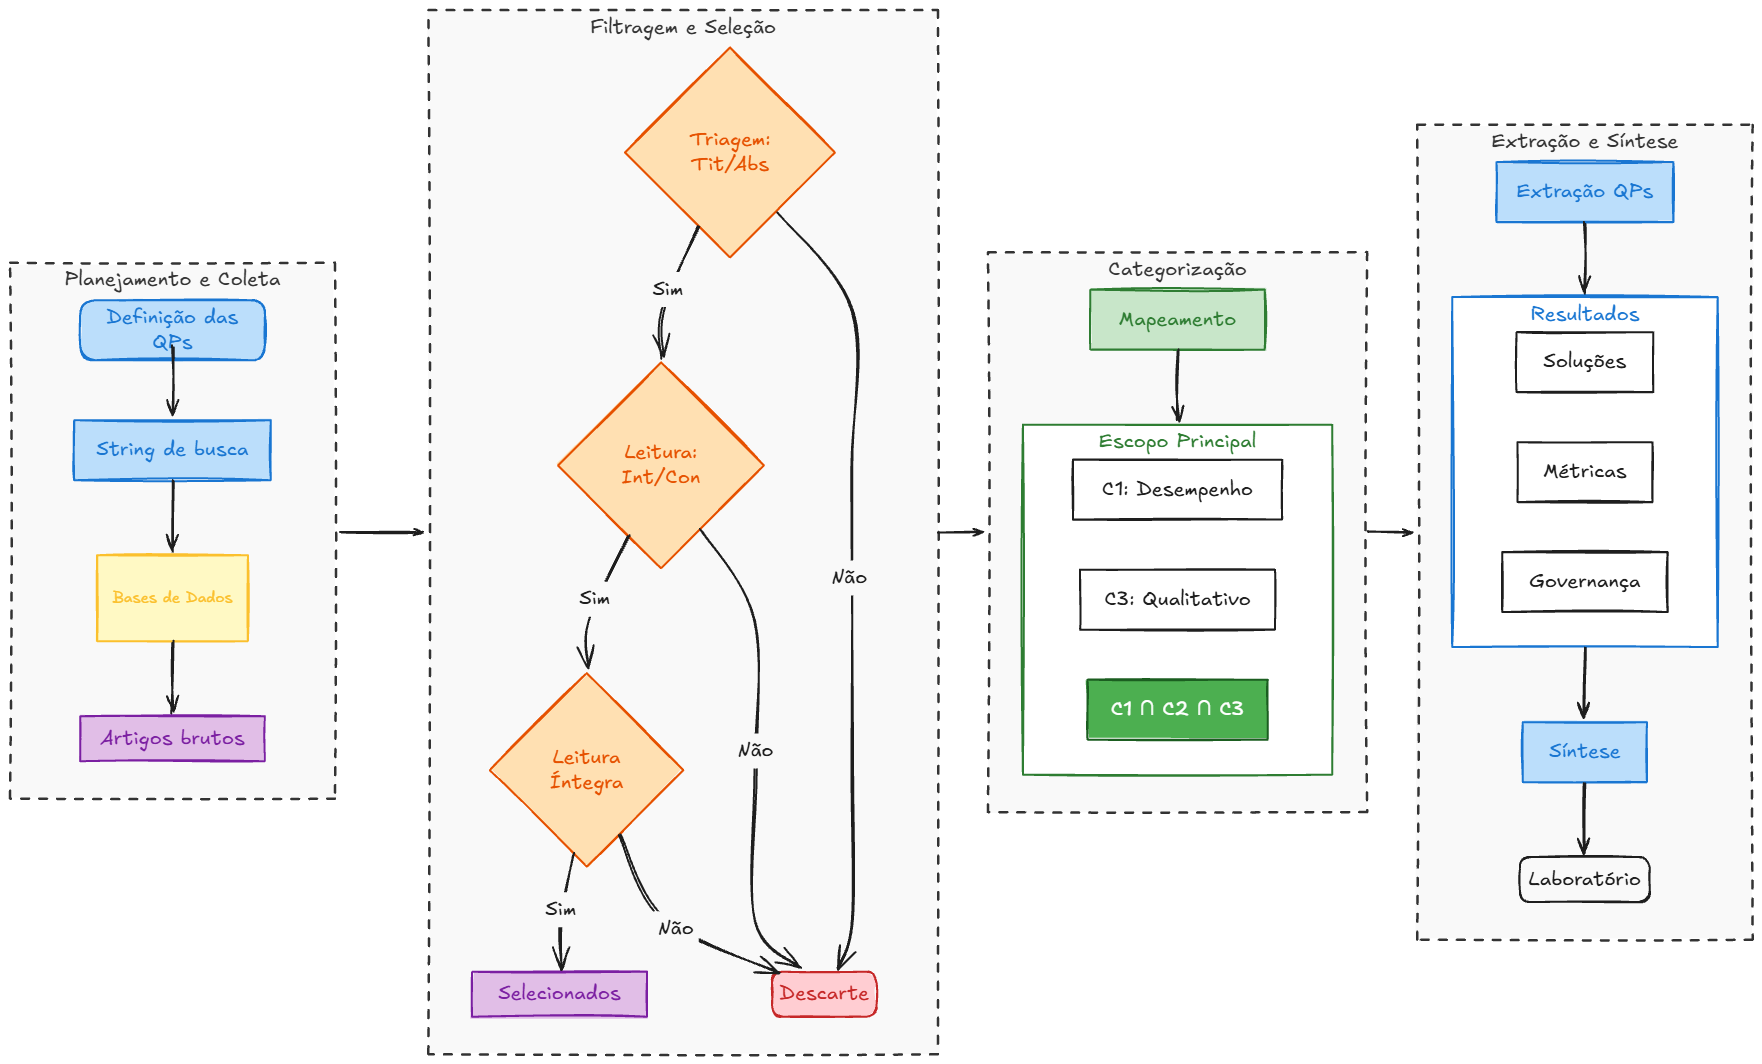
\includegraphics[width=0.8\textwidth]{figuras/mapeamento_sistematico.png}
    \caption{Mapeamento sistemático da literatura}
    \label{fig:mapeamento}
\end{figure}
\begin{enumerate}
    \item \textbf{Questões de pesquisa (QPs):}
    \begin{itemize}
        \item QP1 --- Quais soluções de armazenamento de objetos compatíveis
              com S3 são avaliadas na literatura em contextos de \textit{data lake}
              híbrido ou \textit{on-premises}?
        \item QP2 --- Quais dimensões e métricas são utilizadas para comparar
              soluções de \textit{object storage} na literatura?
        \item QP3 --- Quais fatores relacionados a licenciamento, sustentabilidade
              e governança de dados são considerados na seleção de soluções de
              \textit{object storage}?
        \item QP4 --- Quais limitações ou lacunas são identificadas nos estudos
              existentes sobre avaliação comparativa de soluções de
              \textit{object storage}?
    \end{itemize}

    \item \textbf{String de busca:}
    \begin{center}
    \texttt{("object storage" OR "object store" OR "S3-compatible")}\\
    \texttt{AND}\\
    \texttt{("data lake" OR "hybrid cloud" OR "on-premises" OR "distributed storage")}\\
    \texttt{AND}\\
    \texttt{("comparison" OR "evaluation" OR "benchmark" OR "performance" OR "assessment")}
    \end{center}
    As buscas serão conduzidas nas bases:
    \begin{itemize}
      \item ACM Digital Library
      \item IEEE Xplore
      \item Scopus
      \item Springer Link
      \item Google Scholar
    \end{itemize}
    Com filtro temporal de 2018 a 2026.

    \item \textbf{Critérios de inclusão (CI):}
    \begin{itemize}
        \item CI1 --- Estuda ou avalia ao menos uma solução de armazenamento de
              objetos compatível com S3;
        \item CI2 --- Aborda cenários de nuvem híbrida, \textit{on-premises} ou
              \textit{data lake};
        \item CI3 --- Apresenta métricas quantitativas ou critérios qualitativos
              de avaliação;
        \item CI4 --- Publicado entre 2018 e 2026;
        \item CI5 --- Disponível em texto completo.
    \end{itemize}

    \item \textbf{Critérios de exclusão (CE):}
    \begin{itemize}
        \item CE1 --- Trata exclusivamente de armazenamento em nuvem pública
              proprietária, sem foco em soluções de código aberto;
        \item CE2 --- Foca em \textit{block storage} ou \textit{file storage}
              sem comparação com \textit{object storage};
        \item CE3 --- Não apresenta critérios de avaliação, limitando-se à
              descrição da solução;
        \item CE4 --- Não está escrito em inglês ou português;
        \item CE5 --- Versão anterior de um estudo mais completo já incluído;
        \item CE6 --- Texto completo indisponível;
        \item CE7 --- Publicado antes de 2018.
    \end{itemize}

    \item \textbf{Categorias de análise:} os estudos incluídos serão
    classificados em até três categorias, permitindo a construção de um diagrama
    de Venn que evidencie lacunas na literatura:
    \begin{itemize}
        \item C1 --- Avaliação de desempenho (\textit{throughput}, latência,
              IOPS, consumo de recursos);
        \item C2 --- Compatibilidade e integração (API S3, interoperabilidade
              com AWS/Azure/GCP);
        \item C3 --- Fatores qualitativos (licenciamento, governança,
              sustentabilidade, \textit{vendor lock-in}).
    \end{itemize}
    A interseção de C1, C2 e C3 representará o escopo integral deste trabalho,
    e sua eventual ausência na literatura reforçará a contribuição da pesquisa.
\end{enumerate}

\textbf{Fase 2 --- Seleção e implantação.}
Com base nos resultados do mapeamento sistemático, seleção de ao menos três
soluções de armazenamento de objetos compatíveis com a API S3, incluindo
obrigatoriamente o RustFS, e construção de um ambiente experimental padronizado
para execução dos testes em condições equivalentes para todas as soluções,
incluindo o MinIO.

\textbf{Fase 3 --- Experimentação.}
Execução de operações equivalentes de armazenamento e recuperação de objetos com
conjuntos de dados de diferentes características (datasets em diferentes cenários),
coletando métricas de desempenho, latência, \textit{throughput}, consumo de
recursos e estabilidade. Serão avaliadas também as possibilidades de
interoperabilidade com serviços AWS, Azure e GCP.

\textbf{Fase 4 --- Análise comparativa.}
Consolidação dos resultados quantitativos e qualitativos para comparação das
soluções em relação ao \textit{baseline} (MinIO), segundo desempenho,
compatibilidade com S3, complexidade operacional, custos, modelo de licenciamento,
maturidade do projeto, riscos tecnológicos e sustentabilidade da solução. Os
critérios de comparação serão refinados a partir das dimensões levantadas no
mapeamento sistemático.

\textbf{Observações.} As tecnologias específicas para cada fase serão levantadas
no refinamento da revisão da literatura.

\bibliography{bibliografia}

\end{document}